\chapter{Radial Basis Function Neural Network}
\label{chapter:rbf}
\section{簡介}
Radial Basis Function Network(簡稱RBF網路),圖\ref{fig:RbfNetwork}爲演算法的網路架構圖,其中有三層網路層,分別爲輸入、隱藏層與輸出層。在\ref{fig:PerceptonPa}、\ref{fig:PerceptonPb}情況下,都可以利用一條線兩種不同類別分割,但是在\ref{fig:PerceptonPc}的情況,不能用一條線將兩個類別分離,由此可見這就是Single Perceptron缺點。而RBF這個演算法的優勢在於解決Single Perceptron在某些情況下線性不可切割的問題,可以將不可線性分割的資料集轉換到另一個維度如圖\ref{Fig:RbfTransfer}所示,使得轉換過的資料變成可線性分割的問題。
\begin{figure}[htbp]
	\centering
	\centerline{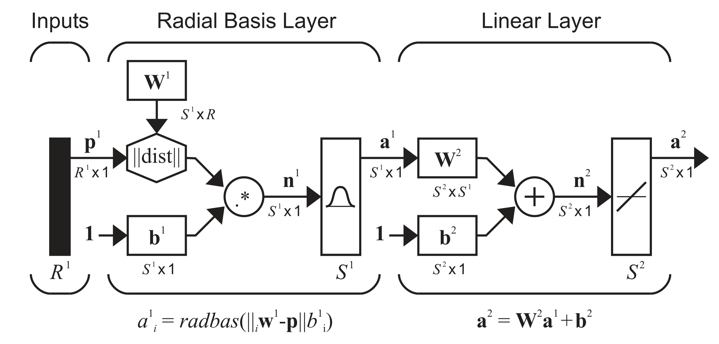
\includegraphics[width=10cm]{pic/rbf_architecture.jpg}}
	\caption{RBF網路架構圖}
	\begin{minipage}{.7\linewidth}
		\footnotesize
		\emph{圖片來源:}取自Function approximation using artificial neural networks
	\end{minipage}
	\label{fig:RbfNetwork}
\end{figure}

\begin{figure}[H]
	\begin{center}
		\begin{tabular}{ccccccccccccc}
			\subfigure[]{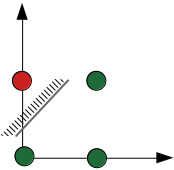
\includegraphics[height=4cm]{./pic/o1PKYrxB.png}\label{fig:PerceptonPa} } \par &
			\subfigure[]{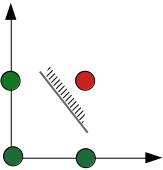
\includegraphics[height=4cm]{./pic/F3BMwBsg.png}\label{fig:PerceptonPb} } \par &
			\subfigure[]{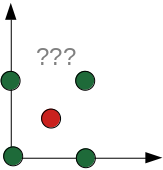
\includegraphics[height=4cm]{./pic/H4K6u1Rx.png}\label{fig:PerceptonPc} } \par   \\
		\end{tabular}
		\caption{可線性分割與不可線性分割示意圖}
		\label{fig:PerceptonProblem}
	\end{center}
\end{figure}


%figure3
\begin{figure}[htbp!]
	\centering
	\subfigure[未轉換過的原資料]{
		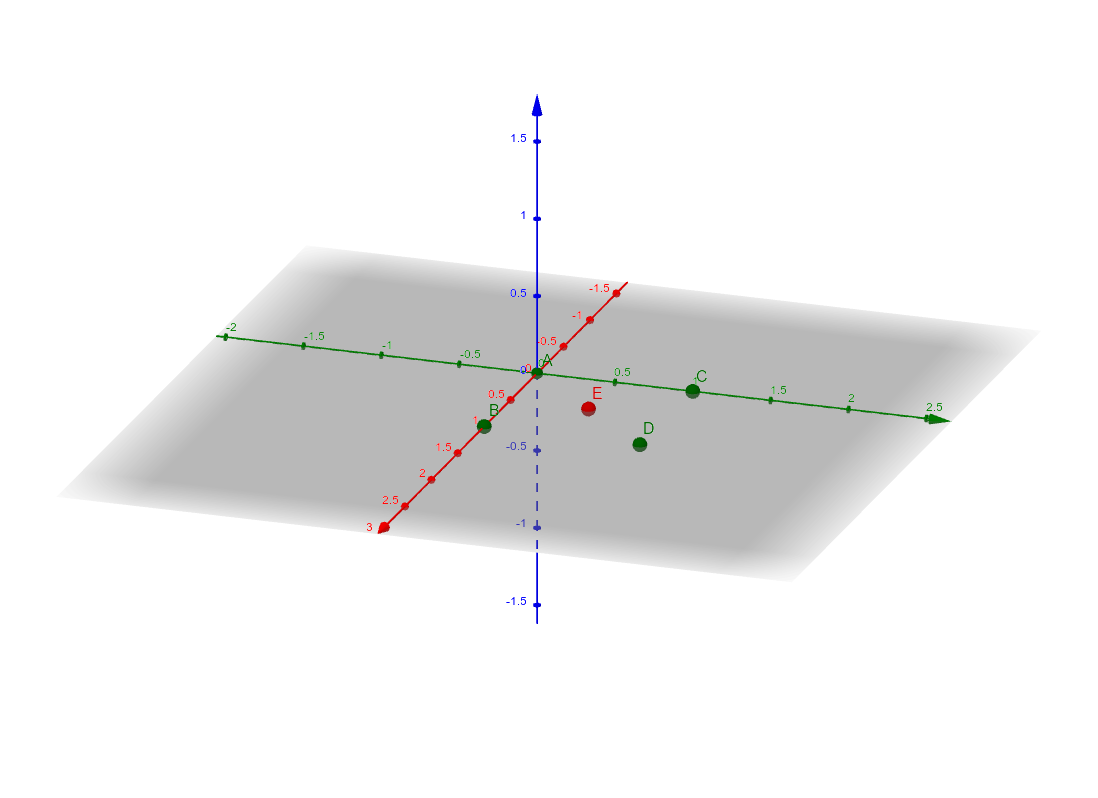
\includegraphics[width=8cm]{./pic/pD17njFW.png}
		%\caption{fig1}
	}

	%	\quad
	\subfigure[經過轉換後的資料]{
		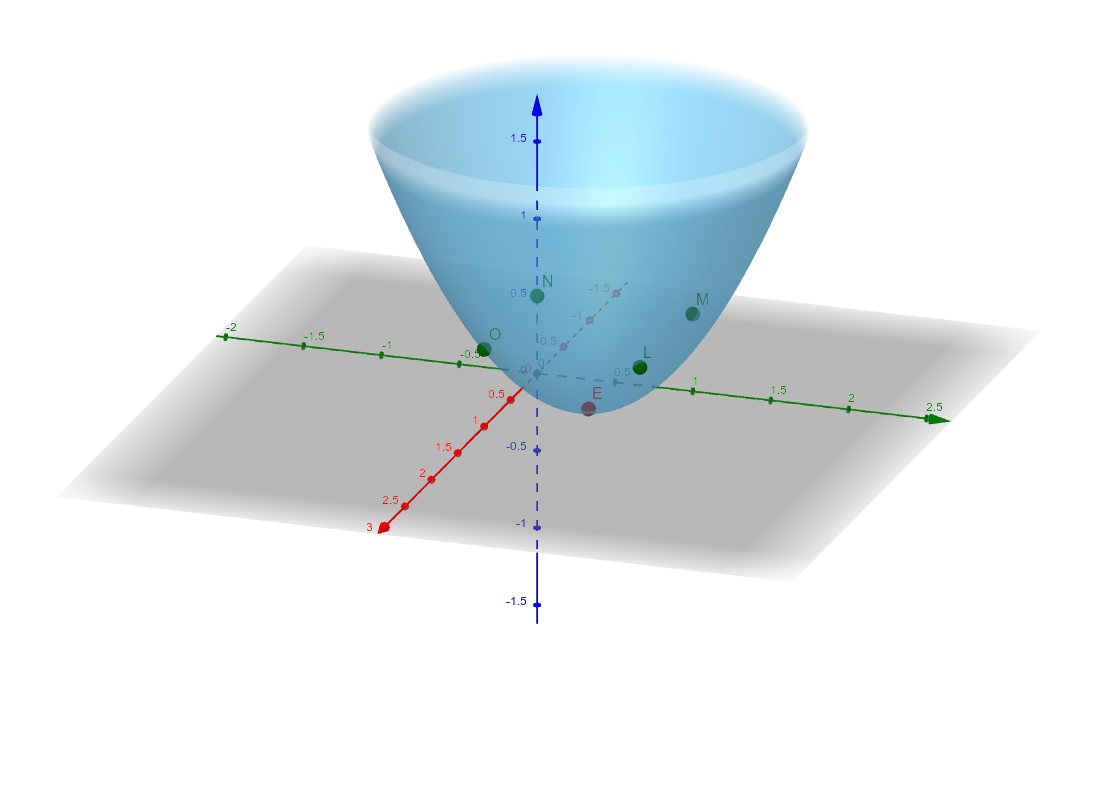
\includegraphics[width=8cm]{./pic/rTd9dG1P.png}
	\label{Fig:RbfTransfer}
	}

	\caption{資料轉換的示意圖}
\end{figure}



\section{Radial Basis Function}
隱層中的Radial Basis Function \(h(.)\)能將資料轉換到另一個維度的函數,以下例子來說明它的運作:

\begin{itemize}
	\item

	      圖\ref{fig:RbfIntroductionNotTransfer}為一個無法線性分割的一維資料集。



	      \begin{figure}[h]
		      \centering
		      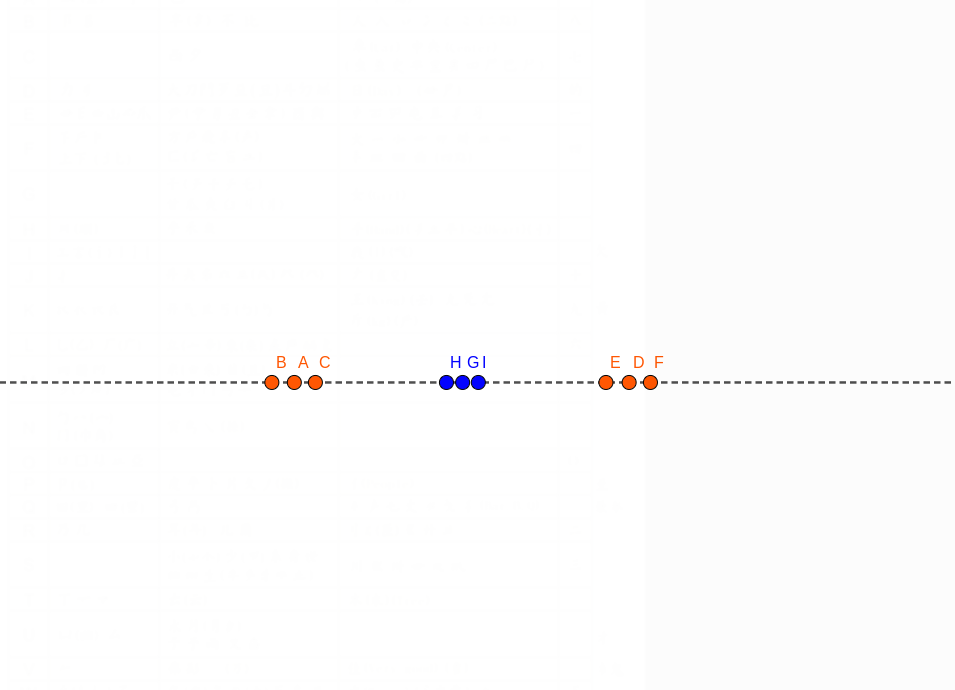
\includegraphics[height=6cm]{./pic/vM4xT9rm.png}
		      \caption{一維資料集}
		      \label{fig:RbfIntroductionNotTransfer}
	      \end{figure}

	\item
	      %%現在我們有一個 \(f(x)\) ,當我們的資料點經過這個函數的轉換,可以發現橘色點都向上移動,而藍色點都向下移動。經過函數轉換的結果後,我們要將這兩個類別進行切割就不難了。
		  根據圖\ref{fig:RbfWithFunction}所示, 資料點經過\(f(x)\)的轉換後,可以觀察到此資料集變成可線性分割。

	      \begin{figure}[h]
		      \centering
		      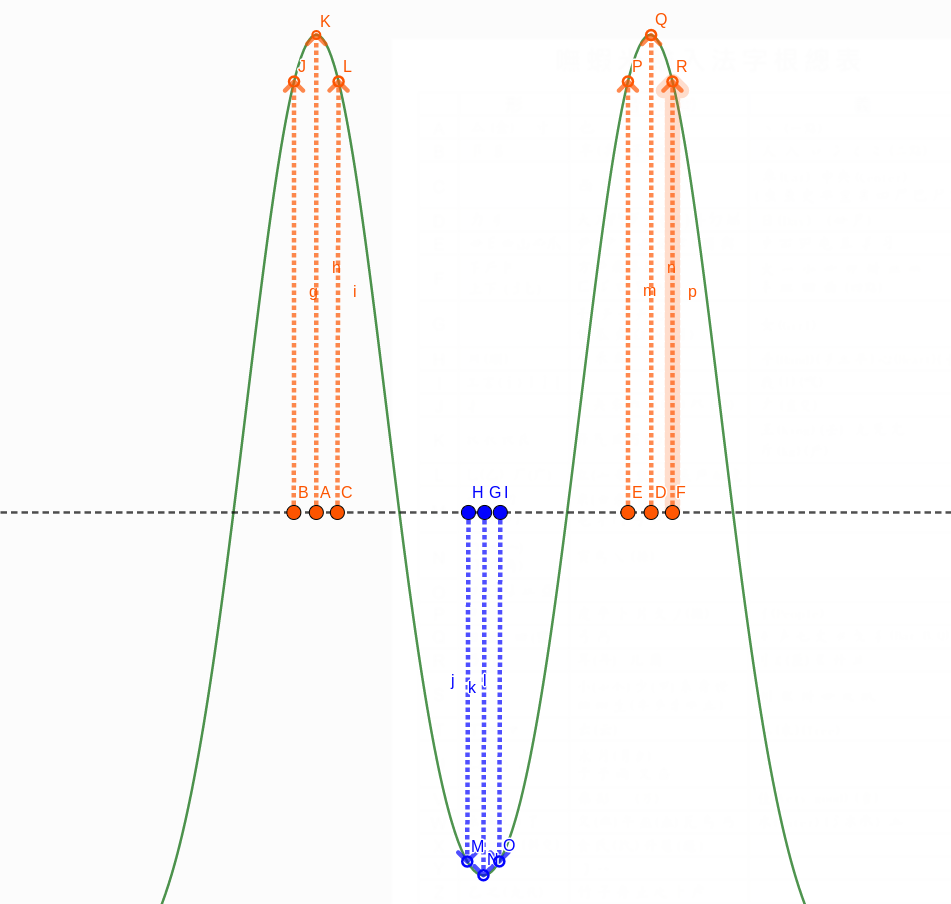
\includegraphics[width=6cm]{./pic/7VM3Lid5.png}
		      \caption{經過 \(f(x)\)轉換的結果 }
		      \label{fig:RbfWithFunction}
	      \end{figure}


	\item
		圖\ref{fig:RbfWithFunction}中的\(f(x)\)是由3個不同的函數與一個常數項所組成,如圖\ref{fig:RbfFunctionAssemble}與(\ref{eqn:RbfFunction})式所示。其中 \(h_1(x)\)、\(h_2(x)\)與\(h_3(x)\)正是 Radial Basis Function,藉由這些函數的組成可以將原本的資料集轉換到另一個維度。

	      \begin{equation}
		      \label{eqn:RbfFunction}
		      f(x)=w_1h_1(x)+w_2h_2(x)+w_3h_3(x)+b
	      \end{equation}

	      \begin{figure}[h]
		      \centering
		      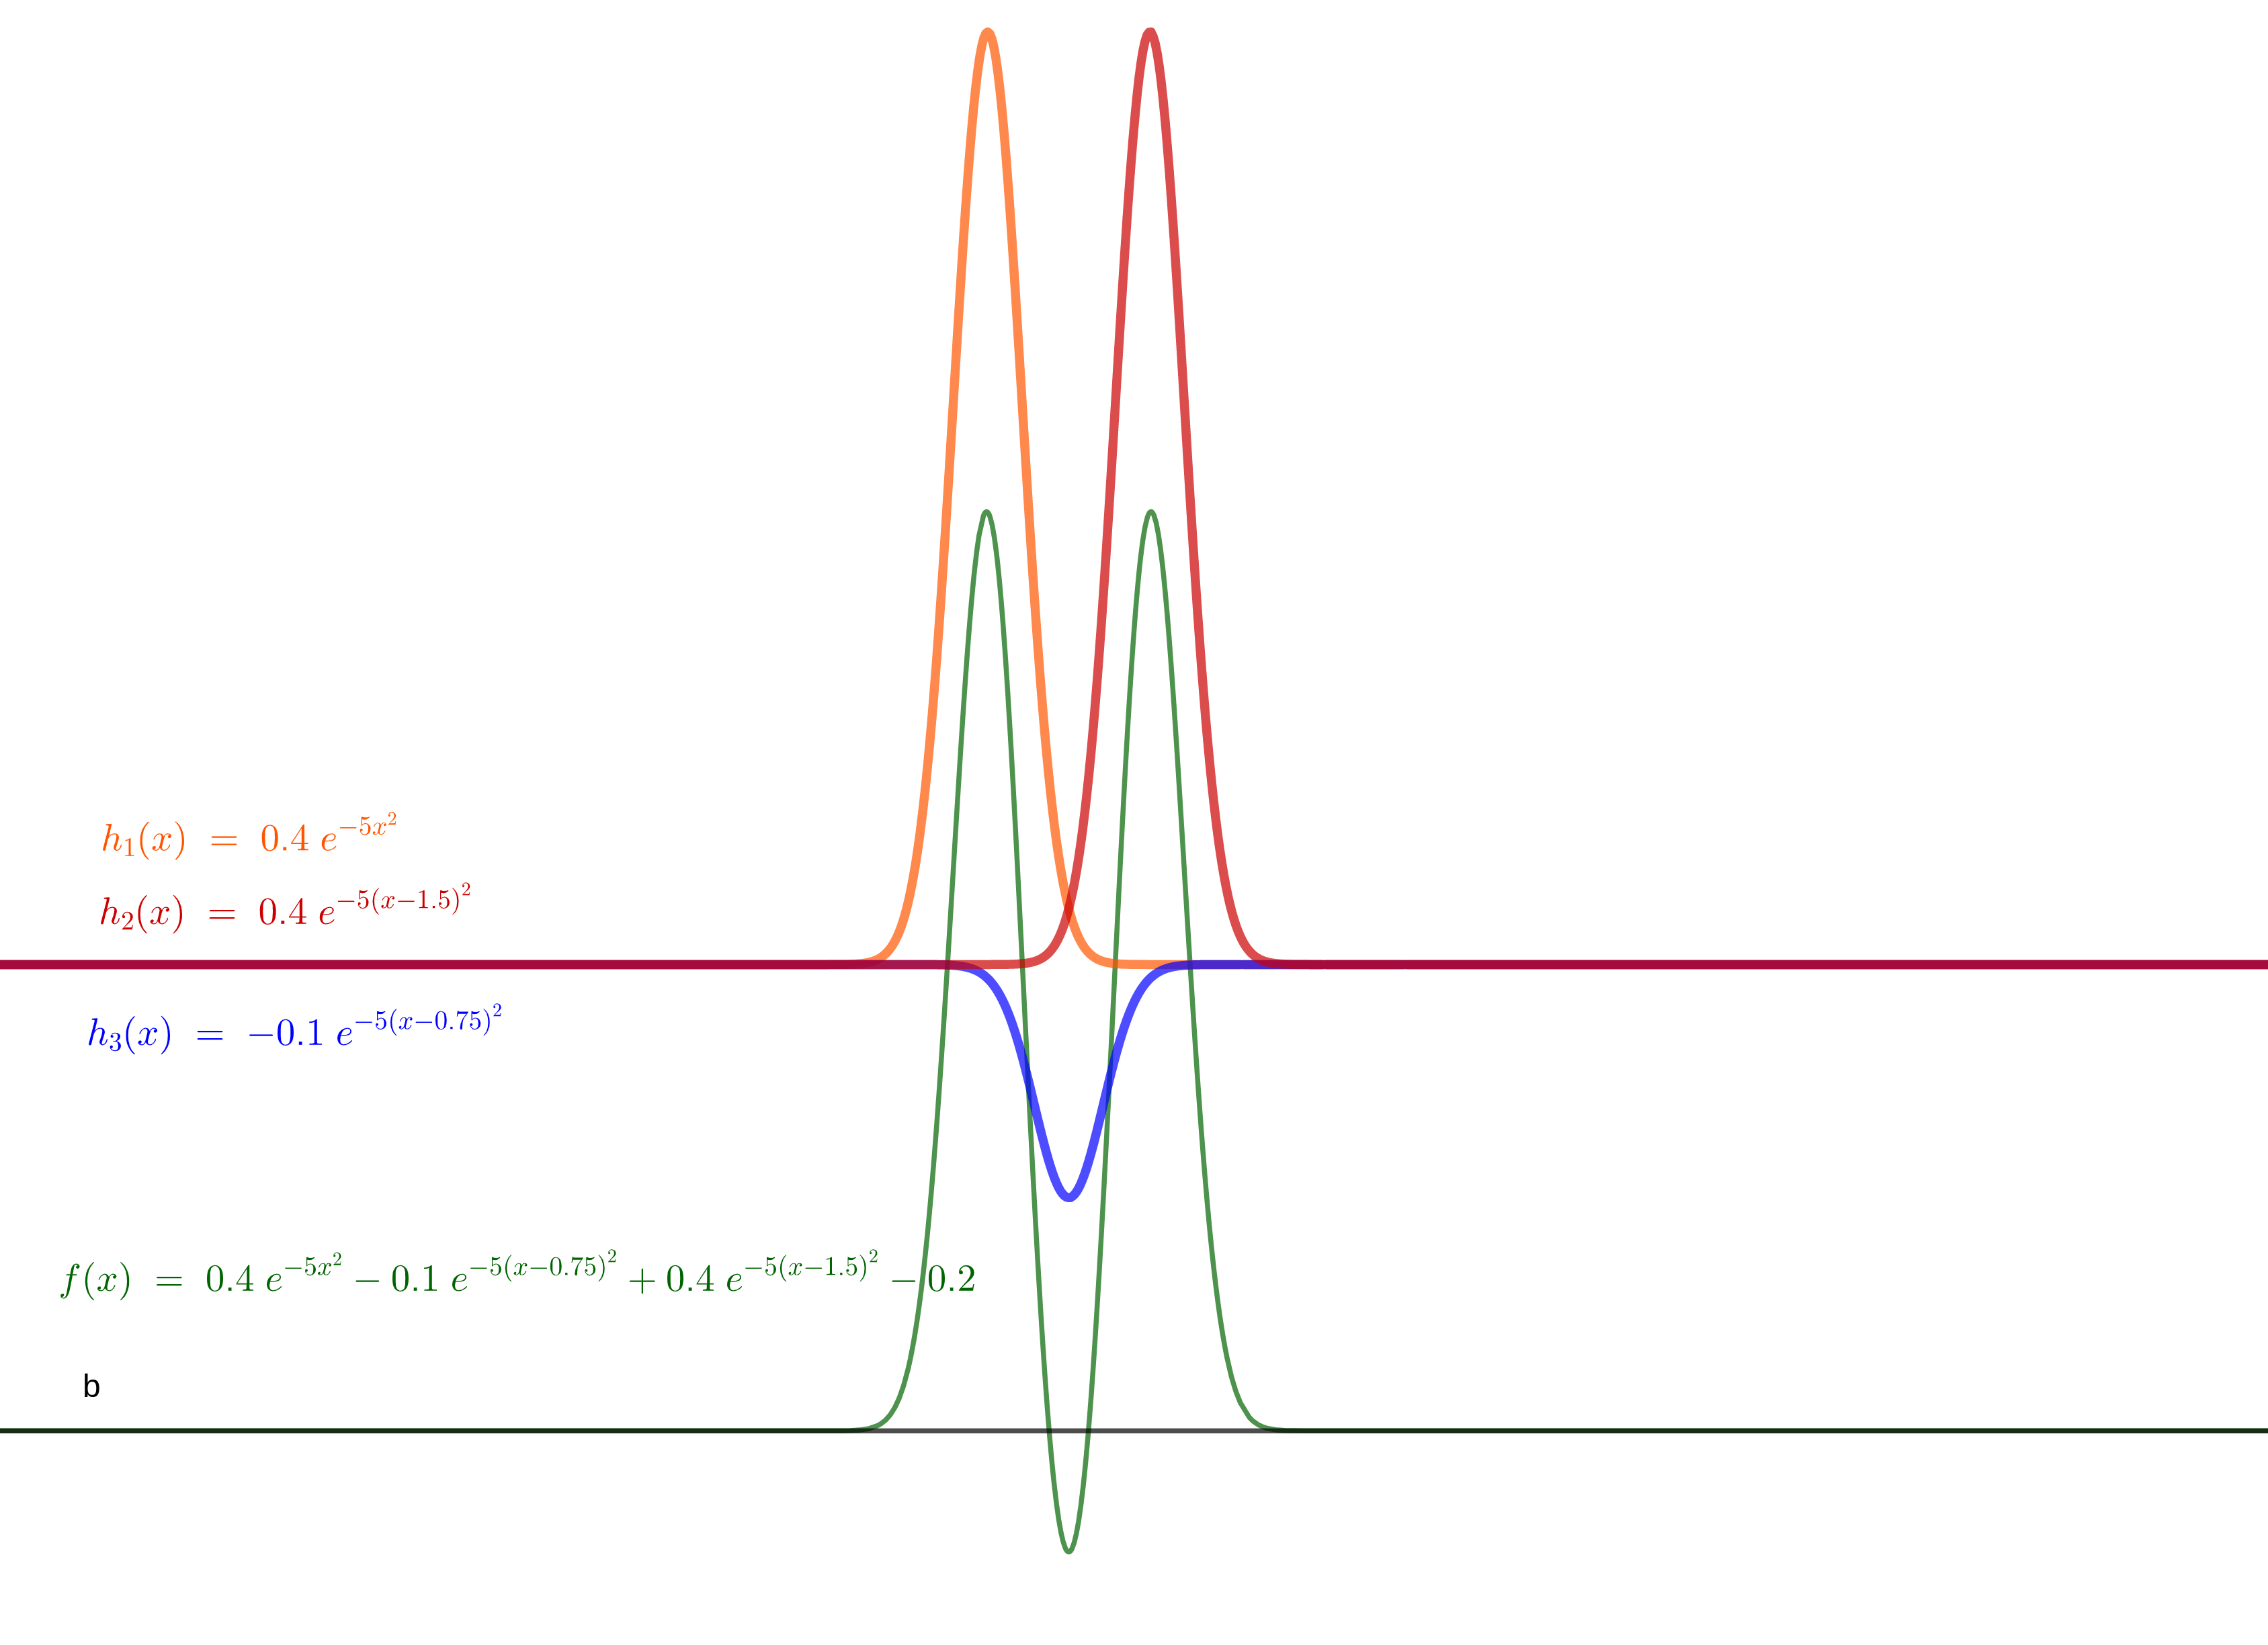
\includegraphics[height=6cm]{./pic/vtYD2no6.png}
		      \caption{\(f(x)\)的組成 }
		      \label{fig:RbfFunctionAssemble}
	      \end{figure}

	\item
	      Radial Basis Function(徑向基函數)會設定一個中心點,並將資料點與這個中心點的距離代入計算輸出結果。
	      式 (\ref{eqn:RadialBasisFunction})與圖\ref{fig:RadialBasisFunction},爲一個中心點為1的高斯函數。
		  從圖\ref{fig:RadialBasisFunction}可以觀察到,離中心點越近能得到越大值,與中心點相關性越大。反之離中心點越遠所得到的值就越小,與中心點的相關性越小。

	      \begin{equation}
		      \label{eqn:RadialBasisFunction}
		      h(x)= e^{-|1-x|^2}
	      \end{equation}

	      \begin{figure}[H]
		      \centering
		      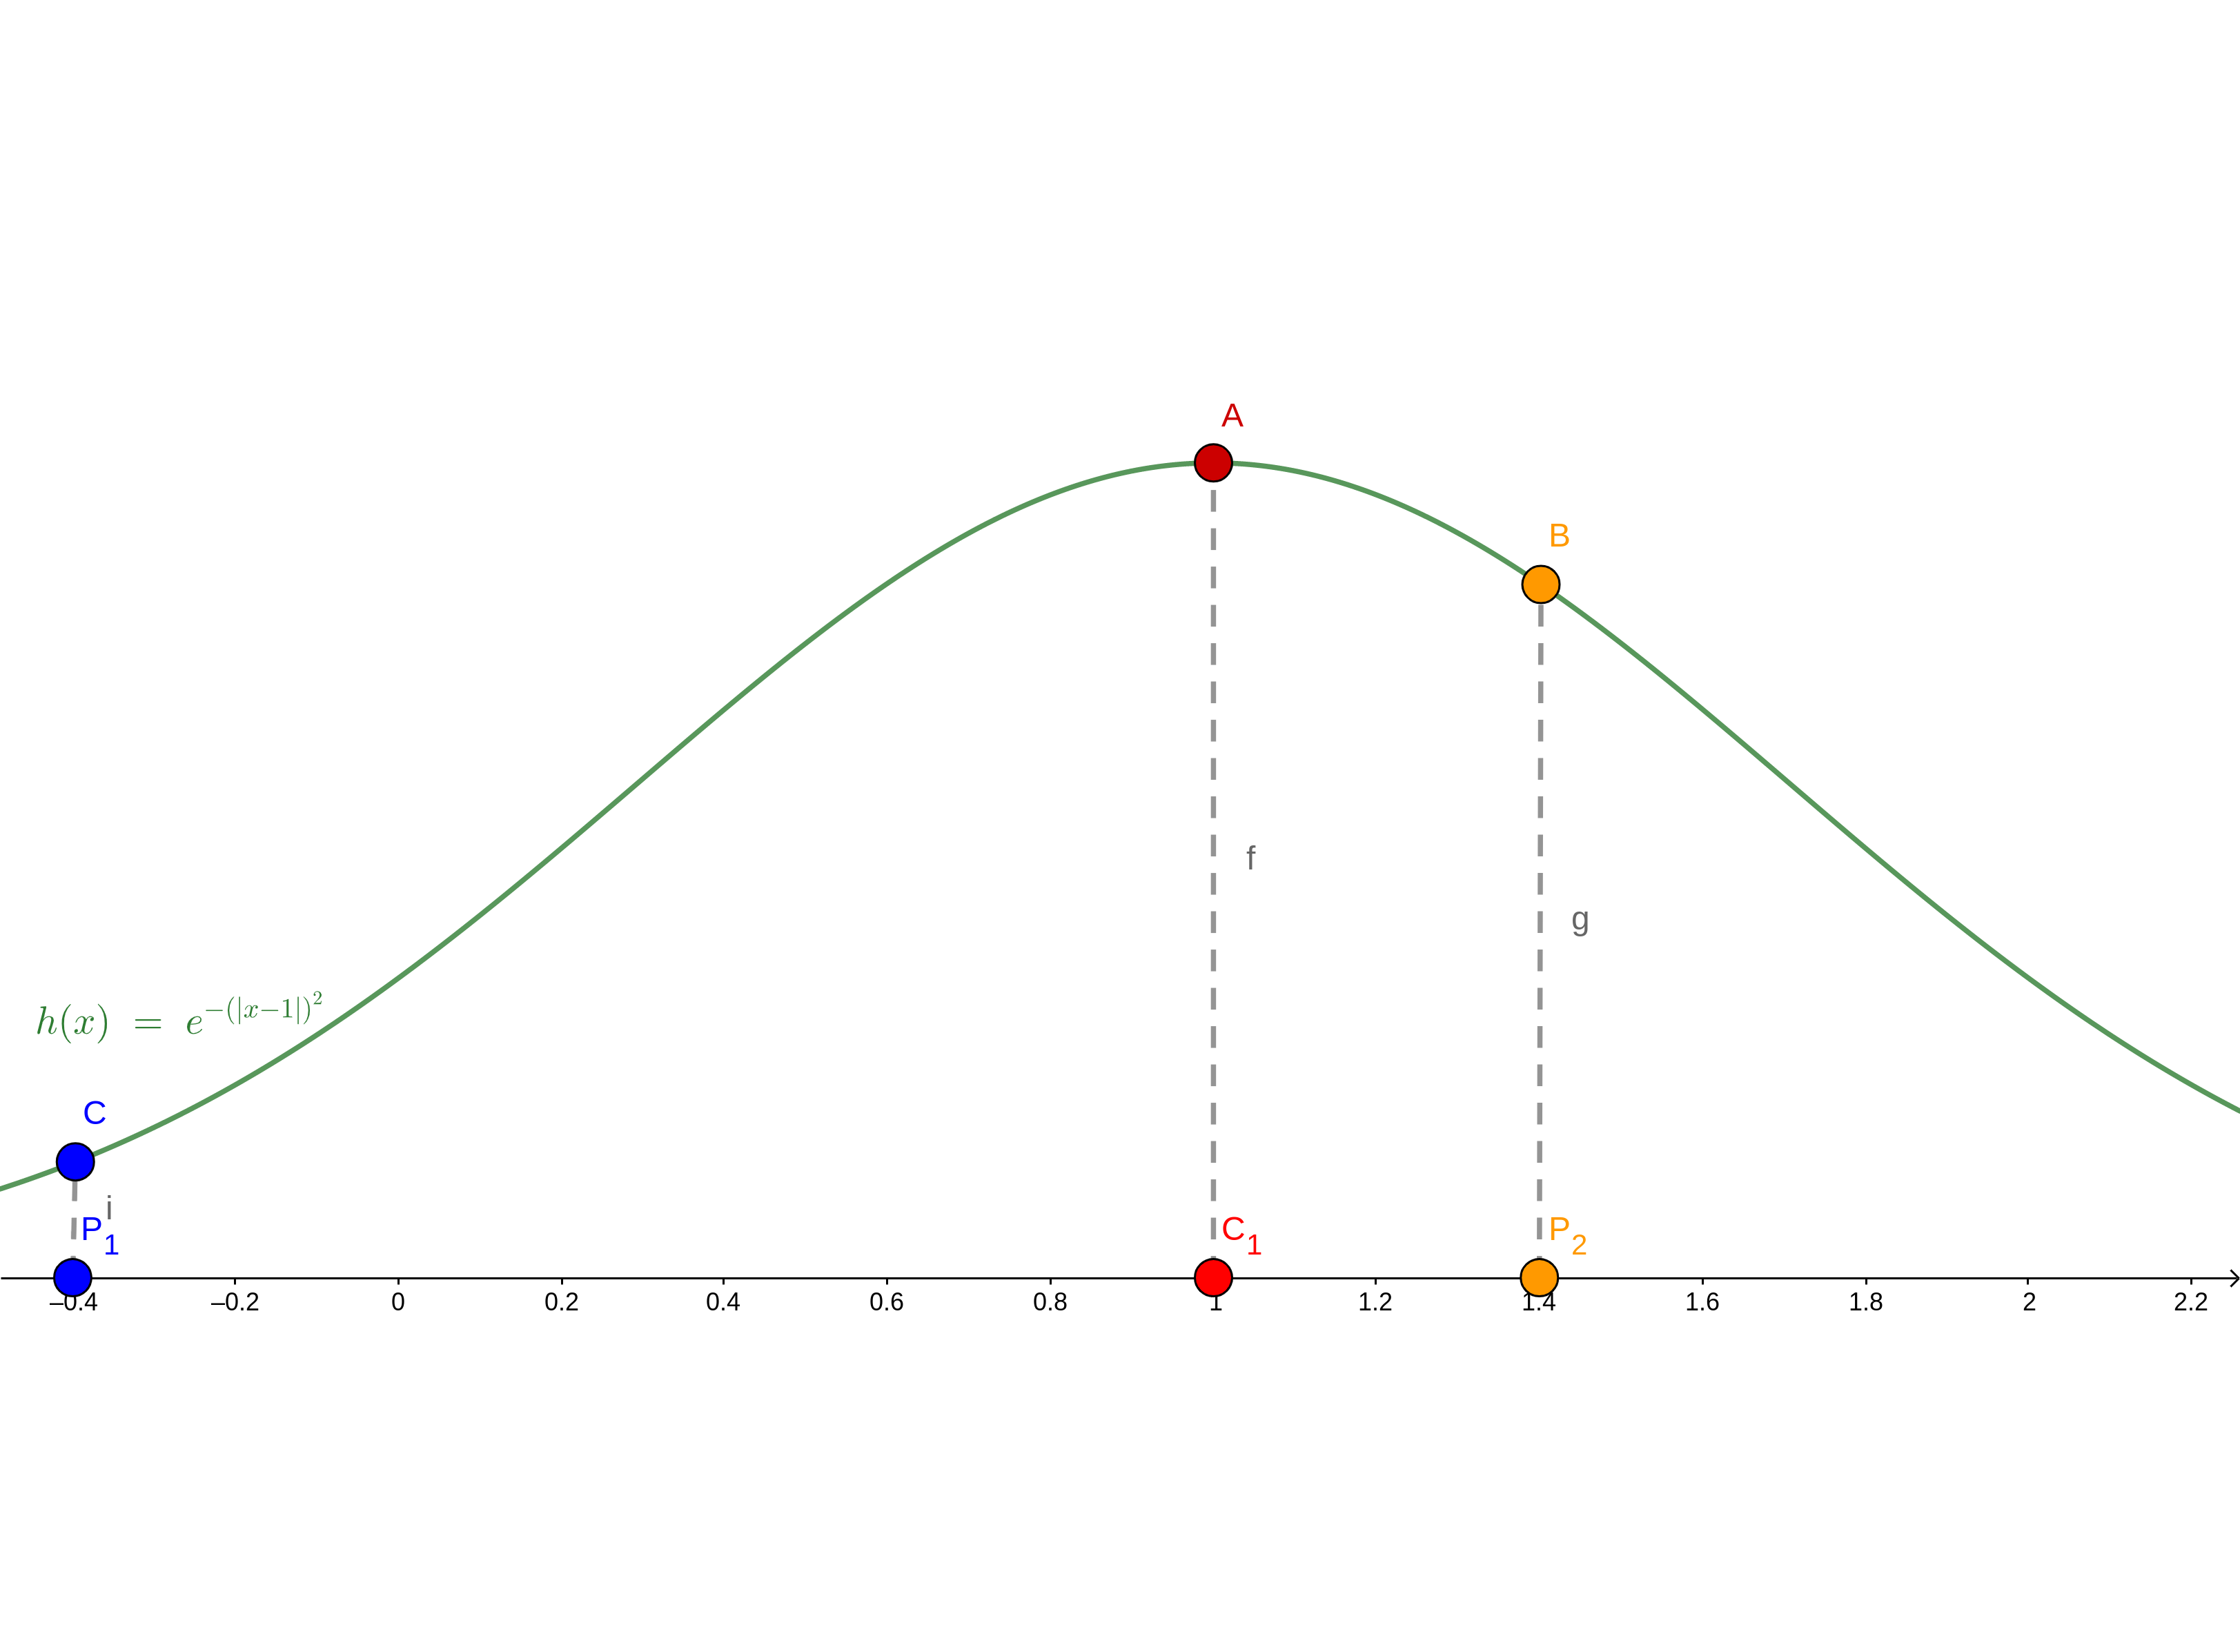
\includegraphics[height=6cm]{./pic/w0KFLczH.png}
		      \caption{}
		      \label{fig:RadialBasisFunction}
	      \end{figure}

\end{itemize}

Rail Basis Function常見的如下表所示:
\\

\begin{table}[h!]
	\centering
	\label{tab:rbf_table}
	\begin{tabular}{ccc}
\toprule
  & RBF的名字 & 方程式 (\(r = ||\mathbf{c-x_i}||\) )   \\ 
\midrule
  & Gaussian Function  & \(h(x)=\phi(r) = e^{-\varepsilon r}\)      \\ \\ 
  & Linear radial Function  & \(h(x)=\phi(r) = r\)      \\ \\
  & Multiquadric   & \(h(x)=\phi(r) = \sqrt{1+(\varepsilon r)^2}\)       \\ \\
  & Inverse quadric  &  \(h(x)=\phi(r) = \frac{1}{1+(\varepsilon r)^2}\)     \\ \\ 
  & Inverse Multiquadric  &  \(h(x)=\phi(r) = \frac{1}{\sqrt{1+(\varepsilon r)^2}}\)     \\
\bottomrule
\end{tabular}

	\caption{常見的Radial Basis Function}
\end{table}




%要被單行註解的文字。


\section{演算法參數定義與流程}




\subsection{參數定義}
\begin{itemize}
	\item
	      輸入向量,\(\mathbf{x} = (x_1,x_2,x_3,....,x_R)\),爲資料集中的一筆資料,輸入向量的 \(R\) 爲資料的特徵數量。
	      %
	\item
	      徑向基層權重,\(\mathbf{W^1} = [\mathbf{c_1,c_2,...,c_j,...c_{S_1}}]^T\),爲一個 \(S_1 \times R \)的矩陣,代表Radial Basis Function中心點集合,這邊的 \(S_1\)代表中心點的數量,而 \(\mathbf{c_j}\)為其中一個中心點 。
	      %
	\item
	      徑向基函數, 定義為\(\{h_1(x), h_2(x),...,h_j(x),....h_{S_1}(x) \}\)  。
	      $h_j(x)=\phi(\mathbf{|c_j-x_i|})$。


	\item
	      輸出層權重, \(\mathbf{W^2}= [\mathbf{w_1,w_2,...,w_k,...,w_{S_2}}]^T\),為一個 \(S_2 \times S_1\) 的矩陣,這邊的 \(S_2\)代表輸出的類別數 。偏移向量為, \(\mathbf{b^2}=(b_1,b_2,....b_{S_2})\)。
	\item
	      輸出向量,\(\mathbf{y}= (y_1,y_2,...,y_k,...y_{S_2})\),其中式 (\ref{eqn:RbfOutputLayer})為每個 \(\mathbf{y_k}\)的計算方式。其實仔細觀察可以發現式(\ref{eqn:RbfOutputLayer})與式(\ref{eqn:RbfFunction})所代表函意相同。

	      \begin{equation}
		      \label{eqn:RbfOutputLayer}
		      \mathbf{y_k}= f(x) = \sum_{i=1}^{S_1}w_{ik}\cdot h_i(x)+b_k
	      \end{equation}
	      %
	\item
	      實際類別, \(T\)。
\end{itemize}

\subsection{流程}

首先初始化 \(\textbf W^1\)  、 \(\textbf W^2\) 與 \(\mathbf{b^2}\) ,其中 \(\mathbf{W^1}\) 的中心點利用kmeans演算法得到,則\(\textbf W^2\) 與 \(\mathbf{b^2}\)爲隨機生成。接著將所有的資料集進行訓練,利用選定的Radial Basis Function計算每筆 \(\mathbf x\)與每個中心點的 \(\{h_1,...,h_{S_1}\}\),並計算其輸出結果 \(\mathbf{y}\),最後透過最小平方法更新 \(\mathbf{W^2}\) 與 \(\mathbf{b}\) 的值。直到達到訓練條件。

\begin{figure}[H]
	\centering
		\resizebox{300pt}{400pt}{
		\begin{tikzpicture}[scale=1]
			\node[draw, rounded corners,align=center ]                        (start)   {初始化參數 \(\mathbf{W^1,W^2,b^2}\) };
			\node[draw,diamond, below=20pt of start,align = center]                        (input_x)  {訓練 \(\mathbf{x}\) 中的\\每一筆資料};
			\node[draw,  aspect=2, below=20pt of input_x, align = center]     (caculate_rbf_layer)  {計算Radial Basis Layer中的\\  \(h_1(x),h_2(x),...,h_j(x),..h_{S_1}(x)\)  };
			\node[draw,  aspect=2, below=20pt of caculate_rbf_layer, align = center]     (caculate_output_layer)  {計算Output Layer中的\\  \(y_1,y_2,...,y_k,..y_{S_2}\)  };
			\node[draw, below=20pt of caculate_output_layer,align = center]                   (update_output_weight)  {比對 \(y_k\)與 \(T\)\\ 接著利用最小平方法計算並更新 \(W^2\)   };
			\node[draw,diamond, below=20pt of update_output_weight,align = center]                         (end_detect)  {判斷是否\\達到結束條件};
			\node[draw, rounded corners, below=20pt of end_detect]  (end)     {End};

			\draw[->] (start)  --coordinate(le) (input_x);
			\draw[->] (input_x) --node[left]{Yes} (caculate_rbf_layer);
			\draw[->] (input_x.west) --node[above]{No}++(-60pt,0)|-(end_detect.west);
			\draw[->] (caculate_rbf_layer) -- (caculate_output_layer);
			\draw[->] (caculate_output_layer) -- (update_output_weight);
			\draw[->] (update_output_weight) -> (end_detect);
			\draw[->] (end_detect) -- node[left]{Yes}(end);
			\draw[->] (end_detect.east) --node[above]{No}++(250pt,0pt)|-(le) ;

		\end{tikzpicture}
	}

	\caption{演算法流程圖}
	\label{fig:AlogrithmWorkflow}
\end{figure}

\section {總結}
圖\ref{fig:RbfOutcome}為一個二維資料進行RBF Neural Network 訓練的結果,從圖中可以發現分別有紅藍兩類,黑色的*則代表各個經徑向基底函數的中心點,經過訓練後可以在圖上畫出一個決策邊界。
從訓練結果可以觀察到RBF Neural Network演算法的優點,能順利將不可線性分割的資料集進行分類,又因為訓練的參數不多,所以短時間就能訓練出不錯的結果。
\newpage
此外,在這個演算法中,中心點的數量與位置會影響訓練效果,數量太多會導致訓練結果過擬合,數量太少則導致訓練結果不理想,而中心點的位置選的不好,即便數量對了,訓練的效果也可能會不好。




\begin{figure}[h]
	\centering
	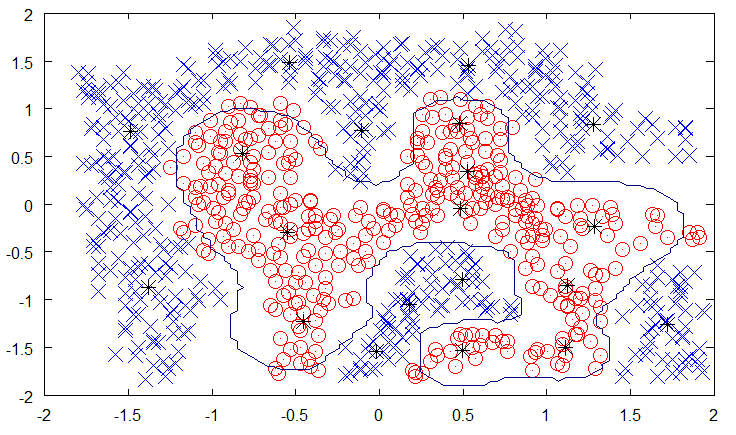
\includegraphics[height=5cm]{./pic/v35Qta6w.png}
	\caption{RBF Network以二維資料訓練的示意圖}

	\begin{minipage}{.7\linewidth}
		\centering
		\footnotesize
		\emph{圖片來源:}取自Radial Basis Function Network (RBFN) Tutorial
	\end{minipage}

	\label{fig:RbfOutcome}
\end{figure}
